\section{Analisi del taglio e della flessione}	
	Come studiato in precedenza, la presenza dell'azione di taglio $\Tx,\Ty$ è sempre associata ad una variazione di momento flettente $\My,\Mx$ per via delle relazioni di equivalenza statica $T_y = \frac{d\Mx}{dz}$ e $T_x = - \frac{d\My}{dz}$. Per come visto a pagina \pageref{eq:sv:equivstatica} alle azioni di taglio sono associate le sole componenti di tensione $\txz,\tyz$ (che determinano delle distorsioni angolari $\gxz,\gyz$).
	
	A differenza di altre casistiche è necessario porre attenzione al fatto che le azioni $T_x,T_y$ e $M_z$ non sono necessariamente disaccoppiate, ossia per il teorema di Betti le azioni di taglio possono produrre un determinato lavoro per gli spostamenti dovuti alla torsione e viceversa. In linea generale queste \textbf{azioni} possono essere \textbf{trattate separatamente} solamente quanto sono energeticamente ortogonali, ossia presentano \textbf{lavoro mutuo nullo}. Questa condizione nella pratica si realizza solamente quando le azioni di taglio $T_x,T_y$ determinano una forza $\ov T = \Tx \vers i + \Ty \vers j$ che passa per il centro di taglio $C$ della sezione.
	
	Risolvere analiticamente in forma chiusa l'analisi al taglio risulta difficile e poco pratica per sezioni complesse, per questo tendenzialmente ci si limita a considerare sezioni a doppia/semplice simmetria, sezioni compatte e/o a spessore sottili, sezioni mono-connesse aperte o pluri-connesse chiuse.
	
	\paragraph{Analisi del taglio} Effettuare delle prove sperimentali di puro taglio è impossibile in quanto, come affermato in precedenza, allo stesso è sempre correlato una variazione di momento flettente.
	\figura{6}{1}{azioni-taglio}{diagramma dell'azione interna di taglio e momento flettente per una trave a sezione rettangolare incernierata a muro e caricata all'estremo opposto.}{azioni-taglio}
	
	Per analizzare dunque la risposta della trave si può dunque pensare di utilizzare, in maniera inversa, il principio di sovrapposizione degli effetti: nota la deformata reale del componente e potendo determinare la deformata a flessione della trave, per sottrazione è possibile ricavare la deformazione a puro taglio, come si può vedere in figura \ref{fig:taglio:schemadeformazione}.
	
	\begin{figure}[bht]
		\centering
		\begin{subfigure}{0.32\linewidth}
			\centering 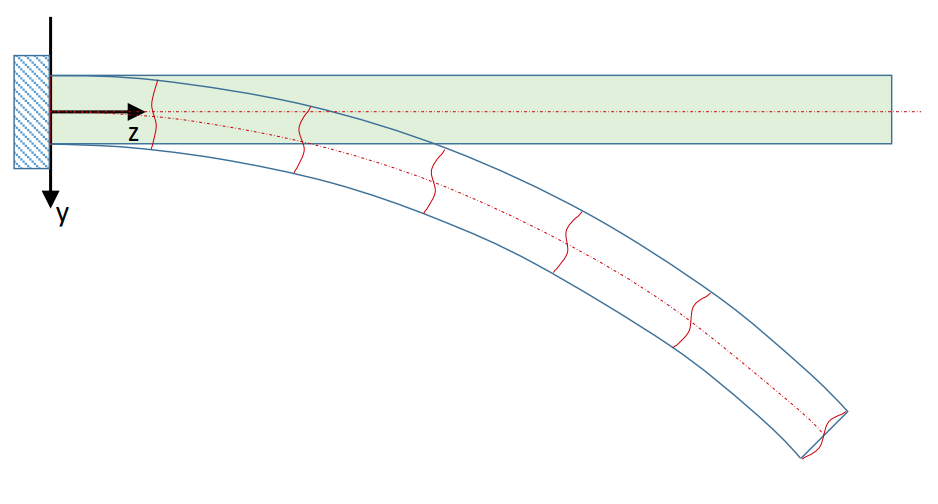
\includegraphics[width=0.9\linewidth]{taglio-a} \caption{}
		\end{subfigure}
		\begin{subfigure}{0.32\linewidth}
			\centering 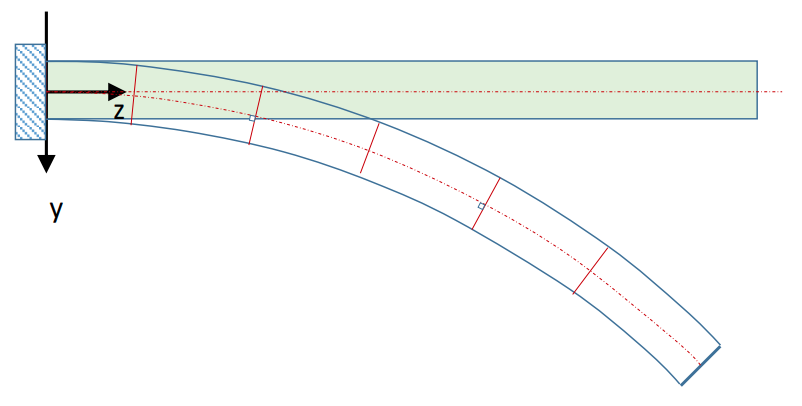
\includegraphics[width=0.9\linewidth]{taglio-b} \caption{}
		\end{subfigure}
		\begin{subfigure}{0.32\linewidth}
			\centering 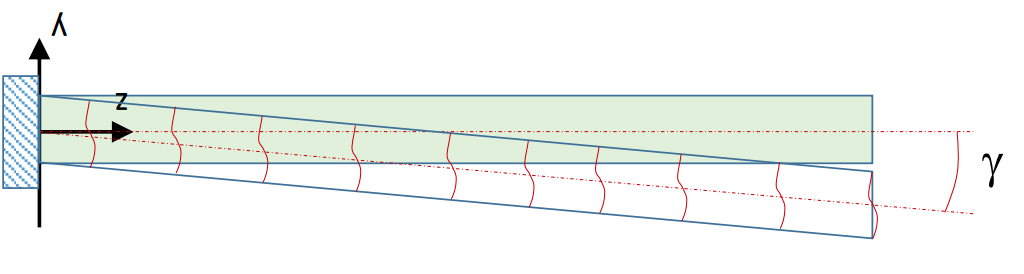
\includegraphics[width=0.9\linewidth]{taglio-c} \caption{}
		\end{subfigure}
		\caption{deformata totale di una trave di una trave sottoposta ad azione di taglio (a), deformata dovuta solamente al momento flettente (b) e conseguente deformata dovuta al solo taglio (c).}
		\label{fig:taglio:schemadeformazione}
	\end{figure}
	
	Si osserva che le sezioni non tendono a rimanere piane, ma sono soggette al fenomeno dell'ingobbamento già visto per la torsione, rappresentata in figura \ref{taglio-d}. In particolare l'azione di taglio non deforma l'asse (che dunque rimane rettilineo) e determina distorsioni angolari $\gxz,\gyz$ che sono nulle sul mantello, mentre risultano essere massime in corrispondenza del centro della sezione stessa.
	
	\figura{6}{1}{taglio-d}{effetto di distorsione della sezione dovuta all'azione di taglio}{taglio-d}
	
	La distorsione angolare è dovuta al fatto che è impedito lo scorrimento relativo tra le fibre longitudinali che compongono la trave, e dunque nascono delle azioni interne (con conseguenti deformazioni) che controbilanciano lo scorrimento. A tal proposito è dunque necessario, per il principio di reciprocità, determinare l'azione normale presente nella trave, che nel caso in questione vale
	\[ \szz = \frac{\Mx(z)}{\Ixx}y = -\frac{\Ty\big(L-z\big)}{\Ixx}y \]
	La presenza dell'azione $\szz$ rende il campo non solenoidale, ossia le linee di flusso della tensione $\ov \tau$ sono aperte.
	
	Per analizzare la distribuzione delle tensioni si farà prima riferimento alla cosiddetta \textbf{tensione retta}, ossia una tensione appartenente ad un asse principale di inerzia (una delle componenti $T_x,T_y$ deve dunque essere nulla), per poi combinare i risultati nella \textbf{tensione deviata}. 
	
	\subsection{Analisi del taglio retto con l'approccio di Jourawsky}
		Per studiare la risposta a taglio di una trave si utilizza l'\textbf{approccio approssimato di Jourawsky} il quale applica un'ipotesi semplificativa sull'andamento delle tensioni partendo da delle considerazioni di equilibrio di un volume elementare.
		
		Per rendere più facile l'analisi si parte a considerare il taglio retto applicato su una sezione a doppio asse di simmetria (che permette dunque di semplificare di fatto i calcoli) come mostrato in figura \ref{taglio-retto-a}.
		
		\figura{3}{2}{taglio-retto-a}{sezione a doppio asse di simmetria sottoposta a taglio retto $T_y$.}{taglio-retto-a}
		
		Le incognite del problema sono di fatto el componenti $\txz$ e $\tyz$ dello stato di tensione della trave; per poter determinare tali valori è necessario considerare le relazioni di equivalenza statica che, per come già visto in precedenza, permettono di affermare che
		\[ T_y = - \frac{d\Mx}{dz} \qquad \textrm e \qquad  \szz = -\frac{\Ty\big(L-z\big)}{\Ixx}y \quad \Rightarrow \quad \pd \szz z = \frac \Ty\Ixx y\]
		Con queste relazioni note è possibile riscrivere l'equilibrio indefinito (già visto a pagina \pageref{sec:sv:equilibrioindefinito}) del campo della trave tramite l'equazione differenziale
		\begin{equation} \label{eq:taglio:temp1}
			\pd \txz x + \pd \tyz y = -\pd \szz z = - \frac \Ty \Ixx y
		\end{equation}
		\begin{nota}
			Questo dimostra la non solenoidalità del campo delle tensioni $\ov \tau$ in quanto si dimostra che $\textrm{div}(\ov \tau) =- \frac \Ty \Ixx y \neq 0$.
		\end{nota}
		
		A questo punto per continuare l'analisi tramite il metodo di Jourawsky si sceglie una corda (la cui lunghezza vale $b(y)$ ) qualsiasi perpendicolare all'asse $y$ dove giace l'azione di taglio, ossia determinata (in funzione della coordinata $y$) dai punti
		\[ P_1 = \left(\frac{b(y)}{2}, y\right) \qquad P_2 = \left(-\frac{b(y)}{2}, y\right) \]
		L'andamento delle tensioni $\txz \parallel \ov P_1\ov P_2$ e $\tyz \perp \ov P_1\ov P_2$ non risulta essere noto a priori, tuttavia è possibile supporre che il loro valore sia pressoché costante, e dunque si determina le media integrale di tali grandezze:
		\[ \tau_{yz,m}= \frac 1 {b(y)} \int_{-b/2}^{b/2} \tyz \, dx \qquad \tau_{xz,m}= \frac 1 {b(y)} \int_{-b/2}^{b/2} \txz \, dx = 0  \]
		\figura{3.5}{2}{taglio-retto-b}{tensioni $\txz,\tyz$ e coordinate generalizzate usate per l'analisi del taglio retto.}{taglio-retto-b}
		
		In particolare essendo la sezione simmetrica e la tensione verso solo l'asse $y$, per l'equivalenza statica con $T_x$ è necessario imporre la media integrale del campo scalare $\txz$ come nulla.
		
		\begin{concetto}
			L'\textbf{ipotesi semplificativa di Jourawsky} si basa sul fatto di considerare il campo $\tyz$ costante lungo tutta la corda della sezione perpendicolare all'asse $y$ e pari al valor medio $\tyz = \tau_{yz,m}$; al contrario il valor medio $\tau_{xz,m}$ deve essere nullo.
		\end{concetto}
		
		A questo punto è necessario determinare un \textit{metodo} per calcolare il valor medio della tensione lungo la corda della sezione. A tal fine si considera l'\textbf{area sottesa alla corda} $A^*$ e il concio elementare che essa genera, come in figura \ref{taglio-retto-c}. Partendo da tale diagramma è possibile osservare come, per reciprocità, la componente di tensione $\tyz$ presenta anche un'azione applicata parallelamente all'asse $z$ (direzione dell'azione $\szz$).
		
		\figura{5}{1.3}{taglio-retto-c}{volume elementare estratto dall'area sottesa $A^*$ alla corda; l'ultima immagine rappresenta anche i conci elementari adiacenti a quello considerato per effettuare il bilancio delle azioni interne.}{taglio-retto-c}
		
		Si può dunque osservare che in corrispondenza della faccia $AB$ agisce una forza $\szz$ (dovuta alle azioni di superficie sul concio elementare), mentre su $CD$ si ha un'azione pari a $\szz + \pd \szz z dz$; in particolare la risultante netta $dN$ dovuta all'azione interna normale può essere calcolata noto che la variazione $\pd \szz z$ coincide, per come visto nell'equazione \ref{eq:taglio:temp1}, con la funzione $-\frac \Ty\Ixx y$ e dunque
		\[ dN = \int_{A^*(y)} \pd \szz z \, dz\, dA = \int_{A^*(y)} \pd Ty \Ixx y \, dz \, dA \]
		
		\begin{concetto}
			Questa forza deve dunque essere contro-bilanciata dall'azione reciproca di $\tyz$ che, in questo caso, risulta valere $dF = \tau_{yz,m} b(y)\, dz$: eguagliando dunque i termini $dN = dF$ è possibile esplicitare il valor medio della componente $\tyz$, che prende il nome di \textbf{tensione di Jourawsky}, dell'area sottesa $A^*$ tramite l'espressione
			\begin{equation} \label{eq:taglio:retto}
				\tau_{yz,m} = \frac{\Ty  }{\Ixx \, b(y)}\int_{A^*} y\, dA  = \frac{\Ty  }{\Ixx \, b(y)} S_x^*
			\end{equation}
		\end{concetto}
		Si può dunque osservare che l'integrale $\int_{A^*}y\,dA = S_x^*$ rappresenta il momento statico dell'area $A^*$ valutato rispetto all'asse $x$; in questa espressione va notato come il rapporto $T_y/\Ixx$ sia una proprietà fissa della trave, mentre $S_x^*/b$ è una funzione dipendente dalla posizione $y$ rispetto alla quale si sceglie di posizionare la corda (infatti variando $y$ varia sia l'area che determina il momento statico, sia in generale la lunghezza della corda stessa).
		\figura{3.5}{2}{taglio-retto-d}{azioni $dN$ dovute alle azioni interne e $dF$ dovute alle azioni di taglio.}{taglio-retto-d}
		
		Avendo considerato la sezione della trave come doppiamente simmetrica, allora è possibile verificare la condizione di componente $\tyz$ nulla al contorno del mantello: tale considerazione è basata sul calcolo del momento statico rispetto alle coordinate massime e minime di $y$, e dunque
		\[ \textrm{per } y = \begin{cases}
			y_{max} \qquad \rightarrow \quad A^* = 0 \qquad \Rightarrow \quad S^* = 0 \qquad \Rightarrow \quad \tau_{yz,m} = 0 \\
			y_{min} \qquad \rightarrow \quad A^* = A \qquad \Rightarrow \quad S^* = 0 \qquad \Rightarrow \quad \tau_{yz,m} = 0 \\
		\end{cases}\]
		
		\paragraph{Componente normale all'azione di taglio} Fino ad ora è stato mostrato il processo che permette di calcolare la tensione $\tyz$, assunta come costante e pari al valore medio, dovuta all'azione di taglio dipendente dalla posizione della corda che si vuole scegliere (il risultato è quello esposto nell'equazione \ref{eq:taglio:retto}). Tuttavia quello che resta da definire è il valore della componente $\txz$ che di fatto dovrà garantire la condizione di tangenza del campo $\ov \tau$ al mantello.
		
		L'espressione di tale componente può essere determinata, partendo dalla tensione di Jourawsky, derivando lungo l'asse $x$ l'espressione \ref{eq:taglio:temp1}: osservando che la componente $\txz$ è indipendente dalla posizione $z$ che si sta considerando, allora per integrazione si determina che
		\[ \textrm{eq \ref{eq:taglio:temp1}}\xrightarrow{\pd {}x } \pd{^2\txz}{x^2} = 0 \qquad \xrightarrow{\textrm{ integrazione }} \quad \txz = A(y) x + B(y)  \]
		A questo punto per determinare i coefficienti $A,B$ dipendenti dalla posizione $y$ della corda è necessario imporre le condizioni al contorno; noto il versore $\vers n_\Gamma = (\alpha_x,\alpha_y)$ normale al mantello imponendo il prodotto scalare $\ov \tau \cdot \vers n_\Gamma$ nullo (condizione di perpendicolarità) è possibile ricavare che
		\[ \txz \alpha_x + \tyz \alpha_y = 0\qquad \Rightarrow \quad \txz = -\frac{2x}{b} \frac{\alpha_y}{\alpha_x} \tyz \]
		
		\paragraph{Generalizzazione} La teoria formulata da Jourawsky si basa di fatto sulla formulazione dell'equilibrio di un volume elementare che in generale può essere determinato da una corda non necessariamente ortogonale all'azione di taglio retto, come si può osservare in figura \ref{taglio-retto-gen}. L'analisi di questo tipo di problema è analoga a quanto visto fino ad ora, tuttavia è necessario considerare il sistema di riferimento ruotato di assi $q,\lambda$ e dunque calcolare la componente
		\[\tlz = \frac{\Ty S_x^*(y)}{\Ixx b(y)}\]
		
		\figura{5}{1.2}{taglio-retto-gen}{analisi degli stati di tensione per corde non perpendicolari all'azione $T_y$.}{taglio-retto-gen}
		
		E' inoltre possibile asserire delle considerazioni sul \textbf{verso} della tensione $\tyz$: scelta infatti l'area $A^*$ se si calcola $\tlz > 0$, allora la tensione è \textbf{entrante nell'area} $A^*$ che si sta considerando, mentre al contrario se $\tyz < 0$ il verso è opposto e dunque uscente dall'area.
		
		
		
		
		
		
		
		
		
		
		
		
		
		
		
		
		